\documentclass{amsart}
\usepackage{amssymb}
\renewcommand{\baselinestretch}{1.5}
\addtolength{\textwidth}{.2in}
\addtolength{\topmargin}{-.5in}
\addtolength{\textheight}{1in}

\usepackage{ifthen}
\usepackage{graphicx}

\newcommand{\versionNum}{$3.2$\ }

\newboolean{InTextBook}
\setboolean{InTextBook}{false}
\newboolean{InWorkBook}
\setboolean{InWorkBook}{false}
\newboolean{InHints}
\setboolean{InHints}{false}

%When this boolean is true (beginning in Section 5.1) we will use the convention
% that $0 \in \Naturals$.  If it is false we will continue to count $1$ as the smallest
%natural number (thus making Giuseppe Peano spin in his grave...)
 
\newboolean{ZeroInNaturals}

%This boolean is used to distinguish the version where we use $\sim$ rather than $\lnot$

\newboolean{LNotIsSim}

%The values of the last two booleans are set in ``switches.tex''

\setboolean{ZeroInNaturals}{true}
\setboolean{LNotIsSim}{false}


\let\savedlnot\lnot
\ifthenelse{\boolean{LNotIsSim}}{\renewcommand{\lnot}{\sim} }{}

%This command puts different amounts of space depending on whether we are
% in the text, the workbook or the hints & solutions manual. 
\newcommand{\twsvspace}[3]{%
 \ifthenelse{\boolean{InTextBook} }{\vspace{#1}}{%
  \ifthenelse{\boolean{InWorkBook} }{\vspace{#2}}{%
   \ifthenelse{\boolean{InHints} }{\vspace{#3}}{} %
   }%
  }%
 }


\newcommand{\wbvfill}{\ifthenelse{\boolean{InWorkBook}}{\vfill}{}}
\newcommand{\wbitemsep}{\ifthenelse{\boolean{InWorkBook} }{\rule[-24pt]{0pt}{60pt}}{}}
\newcommand{\textbookpagebreak}{\ifthenelse{\boolean{InTextBook}}{\newpage}{}}
\newcommand{\workbookpagebreak}{\ifthenelse{\boolean{InWorkBook}}{\newpage}{}}
\newcommand{\hintspagebreak}{\ifthenelse{\boolean{InHints}}{\newpage}{}}

\newcommand{\hint}[1]{\ifthenelse{\boolean{InHints}}{ {\par \hspace{12pt} \color[rgb]{0,0,1} #1 } }{}}
\newcommand{\inlinehint}[1]{\ifthenelse{\boolean{InHints}}{ { \color[rgb]{0,0,1} #1 } }{}}

\newlength{\cwidth}
\newcommand{\cents}{\settowidth{\cwidth}{c}%
\divide\cwidth by2
\advance\cwidth by-.1pt
c\kern-\cwidth
\vrule width .1pt depth.2ex height1.2ex
\kern\cwidth}

\newcommand{\sageprompt}{ {\tt sage$>$} }
\newcommand{\tab}{\rule{20pt}{0pt}}
\newcommand{\blnk}{\rule{1.5pt}{0pt}\rule{.4pt}{1.2pt}\rule{9pt}{.4pt}\rule{.4pt}{1.2pt}\rule{1.5pt}{0pt}}
\newcommand{\suchthat}{\; \rule[-3pt]{.5pt}{13pt} \;}
\newcommand{\divides}{\!\mid\!}
\newcommand{\tdiv}{\; \mbox{div} \;}
\newcommand{\restrict}[2]{#1 \,\rule[-4pt]{.25pt}{14pt}_{\,#2}}
\newcommand{\lcm}[2]{\mbox{lcm} (#1, #2)}
\renewcommand{\gcd}[2]{\mbox{gcd} (#1, #2)}
\newcommand{\Naturals}{{\mathbb N}}
\newcommand{\Integers}{{\mathbb Z}}
\newcommand{\Znoneg}{{\mathbb Z}^{\mbox{\tiny noneg}}}
\ifthenelse{\boolean{ZeroInNaturals}}{%
  \newcommand{\Zplus}{{\mathbb Z}^+} }{%
  \newcommand{\Zplus}{{\mathbb N}} }
\newcommand{\Enoneg}{{\mathbb E}^{\mbox{\tiny noneg}}}
\newcommand{\Qnoneg}{{\mathbb Q}^{\mbox{\tiny noneg}}}
\newcommand{\Rnoneg}{{\mathbb R}^{\mbox{\tiny noneg}}}
\newcommand{\Rationals}{{\mathbb Q}}
\newcommand{\Reals}{{\mathbb R}}
\newcommand{\Complexes}{{\mathbb C}}
%\newcommand{\F2}{{\mathbb F}_{2}}
\newcommand{\relQ}{\mbox{\textsf Q}}
\newcommand{\relR}{\mbox{\textsf R}}
\newcommand{\nrelR}{\mbox{\raisebox{1pt}{$\not$}\rule{1pt}{0pt}{\textsf R}}}
\newcommand{\relS}{\mbox{\textsf S}}
\newcommand{\relA}{\mbox{\textsf A}}
\newcommand{\Dom}[1]{\mbox{Dom}(#1)}
\newcommand{\Cod}[1]{\mbox{Cod}(#1)}
\newcommand{\Rng}[1]{\mbox{Rng}(#1)}

\DeclareMathOperator\caret{\raisebox{1ex}{$\scriptstyle\wedge$}}

\newtheorem*{defi}{Definition}
\newtheorem*{exer}{Exercise}
\newtheorem{thm}{Theorem}[section]
\newtheorem*{thm*}{Theorem}
\newtheorem{lem}[thm]{Lemma}
\newtheorem*{lem*}{Lemma}
\newtheorem{cor}{Corollary}
\newtheorem{conj}{Conjecture}

\renewenvironment{proof}%
{\begin{quote} \emph{Proof:} }%
{\rule{0pt}{0pt} \newline \rule{0pt}{15pt} \hfill Q.E.D. \end{quote}}


\addtolength{\abovedisplayskip}{0pt}
\addtolength{\belowdisplayskip}{24pt}
\addtolength{\abovedisplayshortskip}{0pt}
\addtolength{\belowdisplayshortskip}{48pt}

\newcommand{\vsp}{\rule[-12pt]{0pt}{48pt}}

\begin{document}
\thispagestyle{empty}

\centerline{\Large Activity 29 -- Introduction to Proof}
\centerline{\large relations}

\bigskip
\Large


\begin{enumerate}
\item There is a relation from the set of people to the set of colors that can be defined loosely by: $x\relR y$ if and only if $x$'s favorite color is $y$.  Suppose the set of people is just $\{ Abby, Bob, Cindy, Dave, Ella\} $.  Further, suppose that Bob and Ella both like blue, Abby and Cindy like pink, and Dave prefers green.
Draw this relation using a Venn diagram with arrows.

\vfill

\newpage

\item Below is the Venn-diagram-with-arrows picture for a small subset of the ``people and the cheeses they like'' relation.  
\bigskip

\centerline{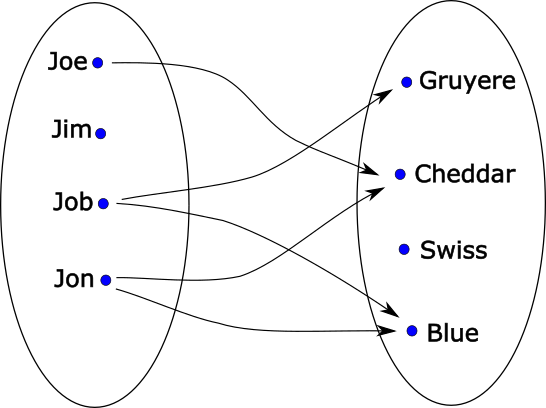
\includegraphics[scale=.5]{relation_pic.png}}
\medskip

Who doesn't like any cheese?  What disgusting cheese is not liked by anyone? What changes would need to be made to this scenario to produce a relation that was a function?

\vfill

\item Write the relation in the last problem as a set of ordered pairs.

\vfill

\newpage

\item Define a relation on $\Reals$ by $x \relR y \; \iff x^2 = y^2$.   Use set-builder notation to write $\relR$ as a set of ordered pairs and sketch a graph of $\relR$ as a subset of the Cartesian plane.

\vfill


\item Define a relation on $\Reals$ by $x \relR y \; \iff x^2 - y^2 \; = \; 1$. Sketch a graph of $\relR$ as a subset of the Cartesian plane.

\vfill

\newpage

\item Consider the following set of trigonometric functions:

\[ A \; = \; \{ \cos{(x)}, \sin{(x)}, -\cos{(x)}, -\sin{(x)} \}. \]

Give the digraph (with vertex set $A$) of the relation 

\[ \relR \; = \; \{ (f(x),g(x) ) \suchthat g(x) = f'(x) \}. \]

\vfill

\end{enumerate}


\end{document}
